\section{General data}

Figure \ref{F_market_cap} depicts the percentage of market capitalization for major cryptocurrencies in relation to the total market capitalization of the cryptocurrency market. The figure showcases the prominent dominance of Bitcoin and Ethereum, which collectively account for nearly 60\% of the cryptocurrency market. The third most important cryptocurrency in market capitalization, Tether (USDT), is a \emph{stable coin} following the value of the US dollar and only accounts for 8\% of the whole market.
\begin{figure*}[ht]
\centering
 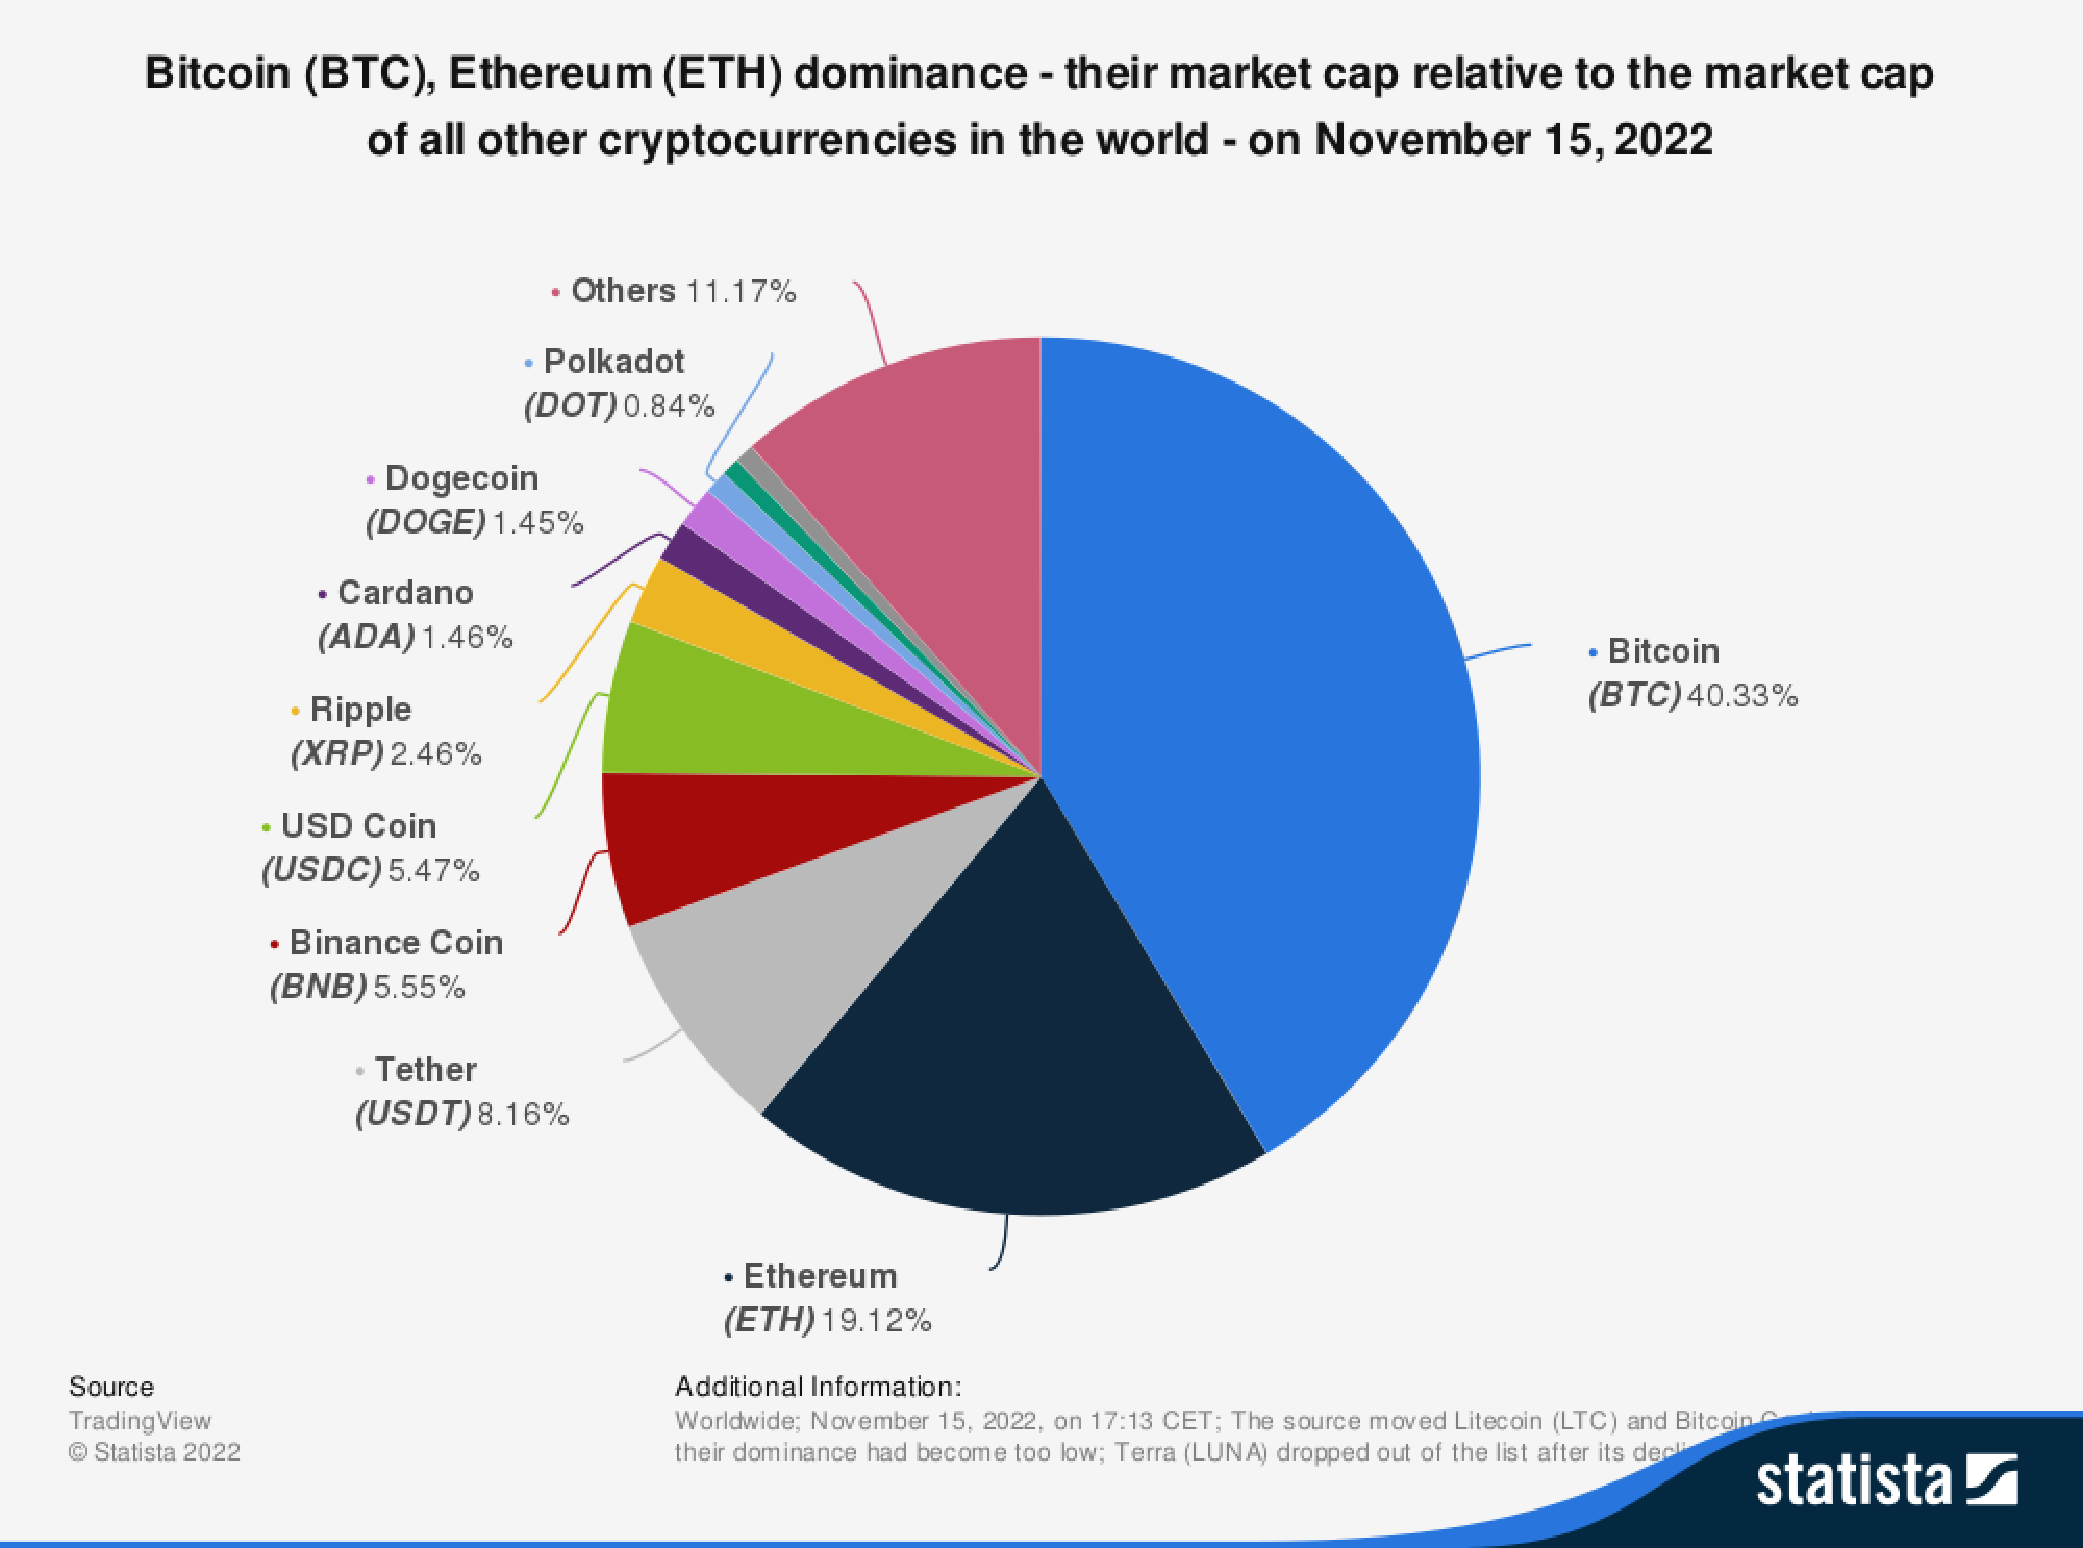
\includegraphics[scale=0.33]{Images/market_dominance.pdf}
\caption{Bitcoin (BTC), Ethereum (ETH) dominance - their market cap relative to the market cap of all other cryptocurrencies in the world - on November 15, 2022 - Statista \cite{tradingview2022}}
\label{F_market_cap}
\end{figure*}

\section{Energy consumption}

Cryptocurrencies based on proof of work, such as BTC, are known for their high electricity consumption. Elements of comparison 
are provided in this section to quantify the actual energy consumption. From the first figure (Figure \ref{F_btc_visa_energy}),
it appears that Bitcoin is consuming more electricity for one transaction, than the Visa network \emph{for 400.000 transactions}. The second figure (Figure 
\ref{F_countries_btc_energy}) highlights the energy consumption of BTC compared to entire countries. Notably, BTC consumes more electricity yearly, that Czechia 
alone.
\begin{figure*}[ht]
    \centering
     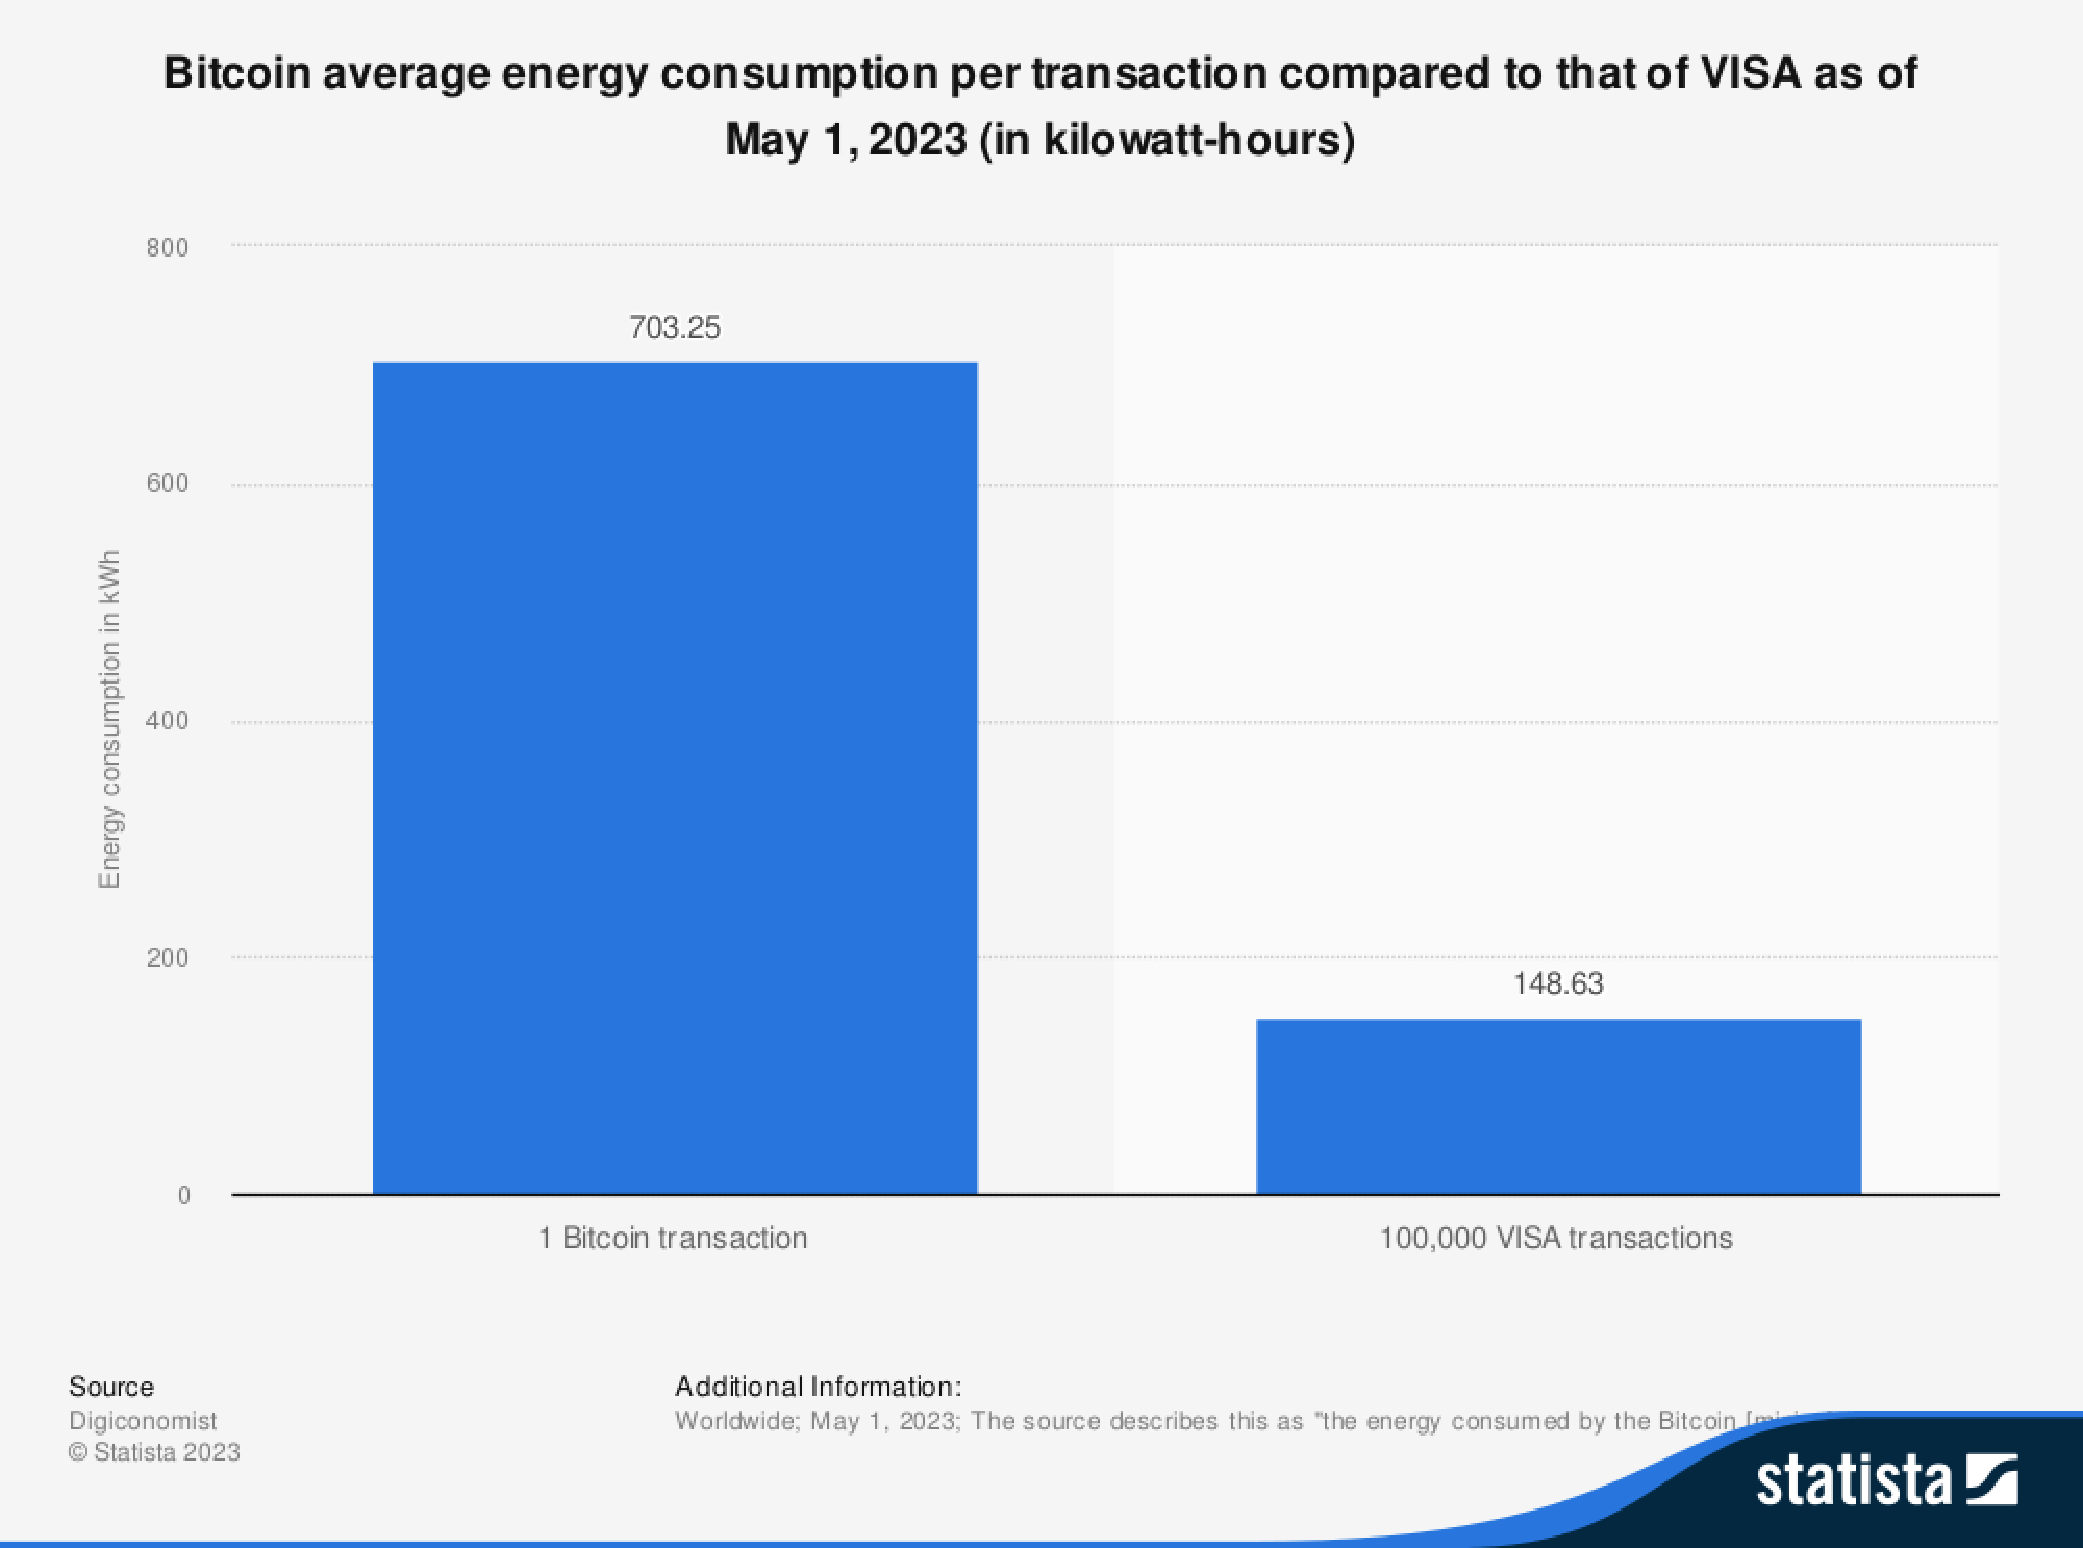
\includegraphics[scale=0.33]{Images/btc_vs_visa_energy.pdf}
    \caption{Bitcoin average energy consumption per transaction compared to that of VISA as of May 1, 2023 in kilowatt-hours - Statista \cite{Digiconomist2023}}
    \label{F_btc_visa_energy}
    \end{figure*}

    \begin{figure*}
        \centering
         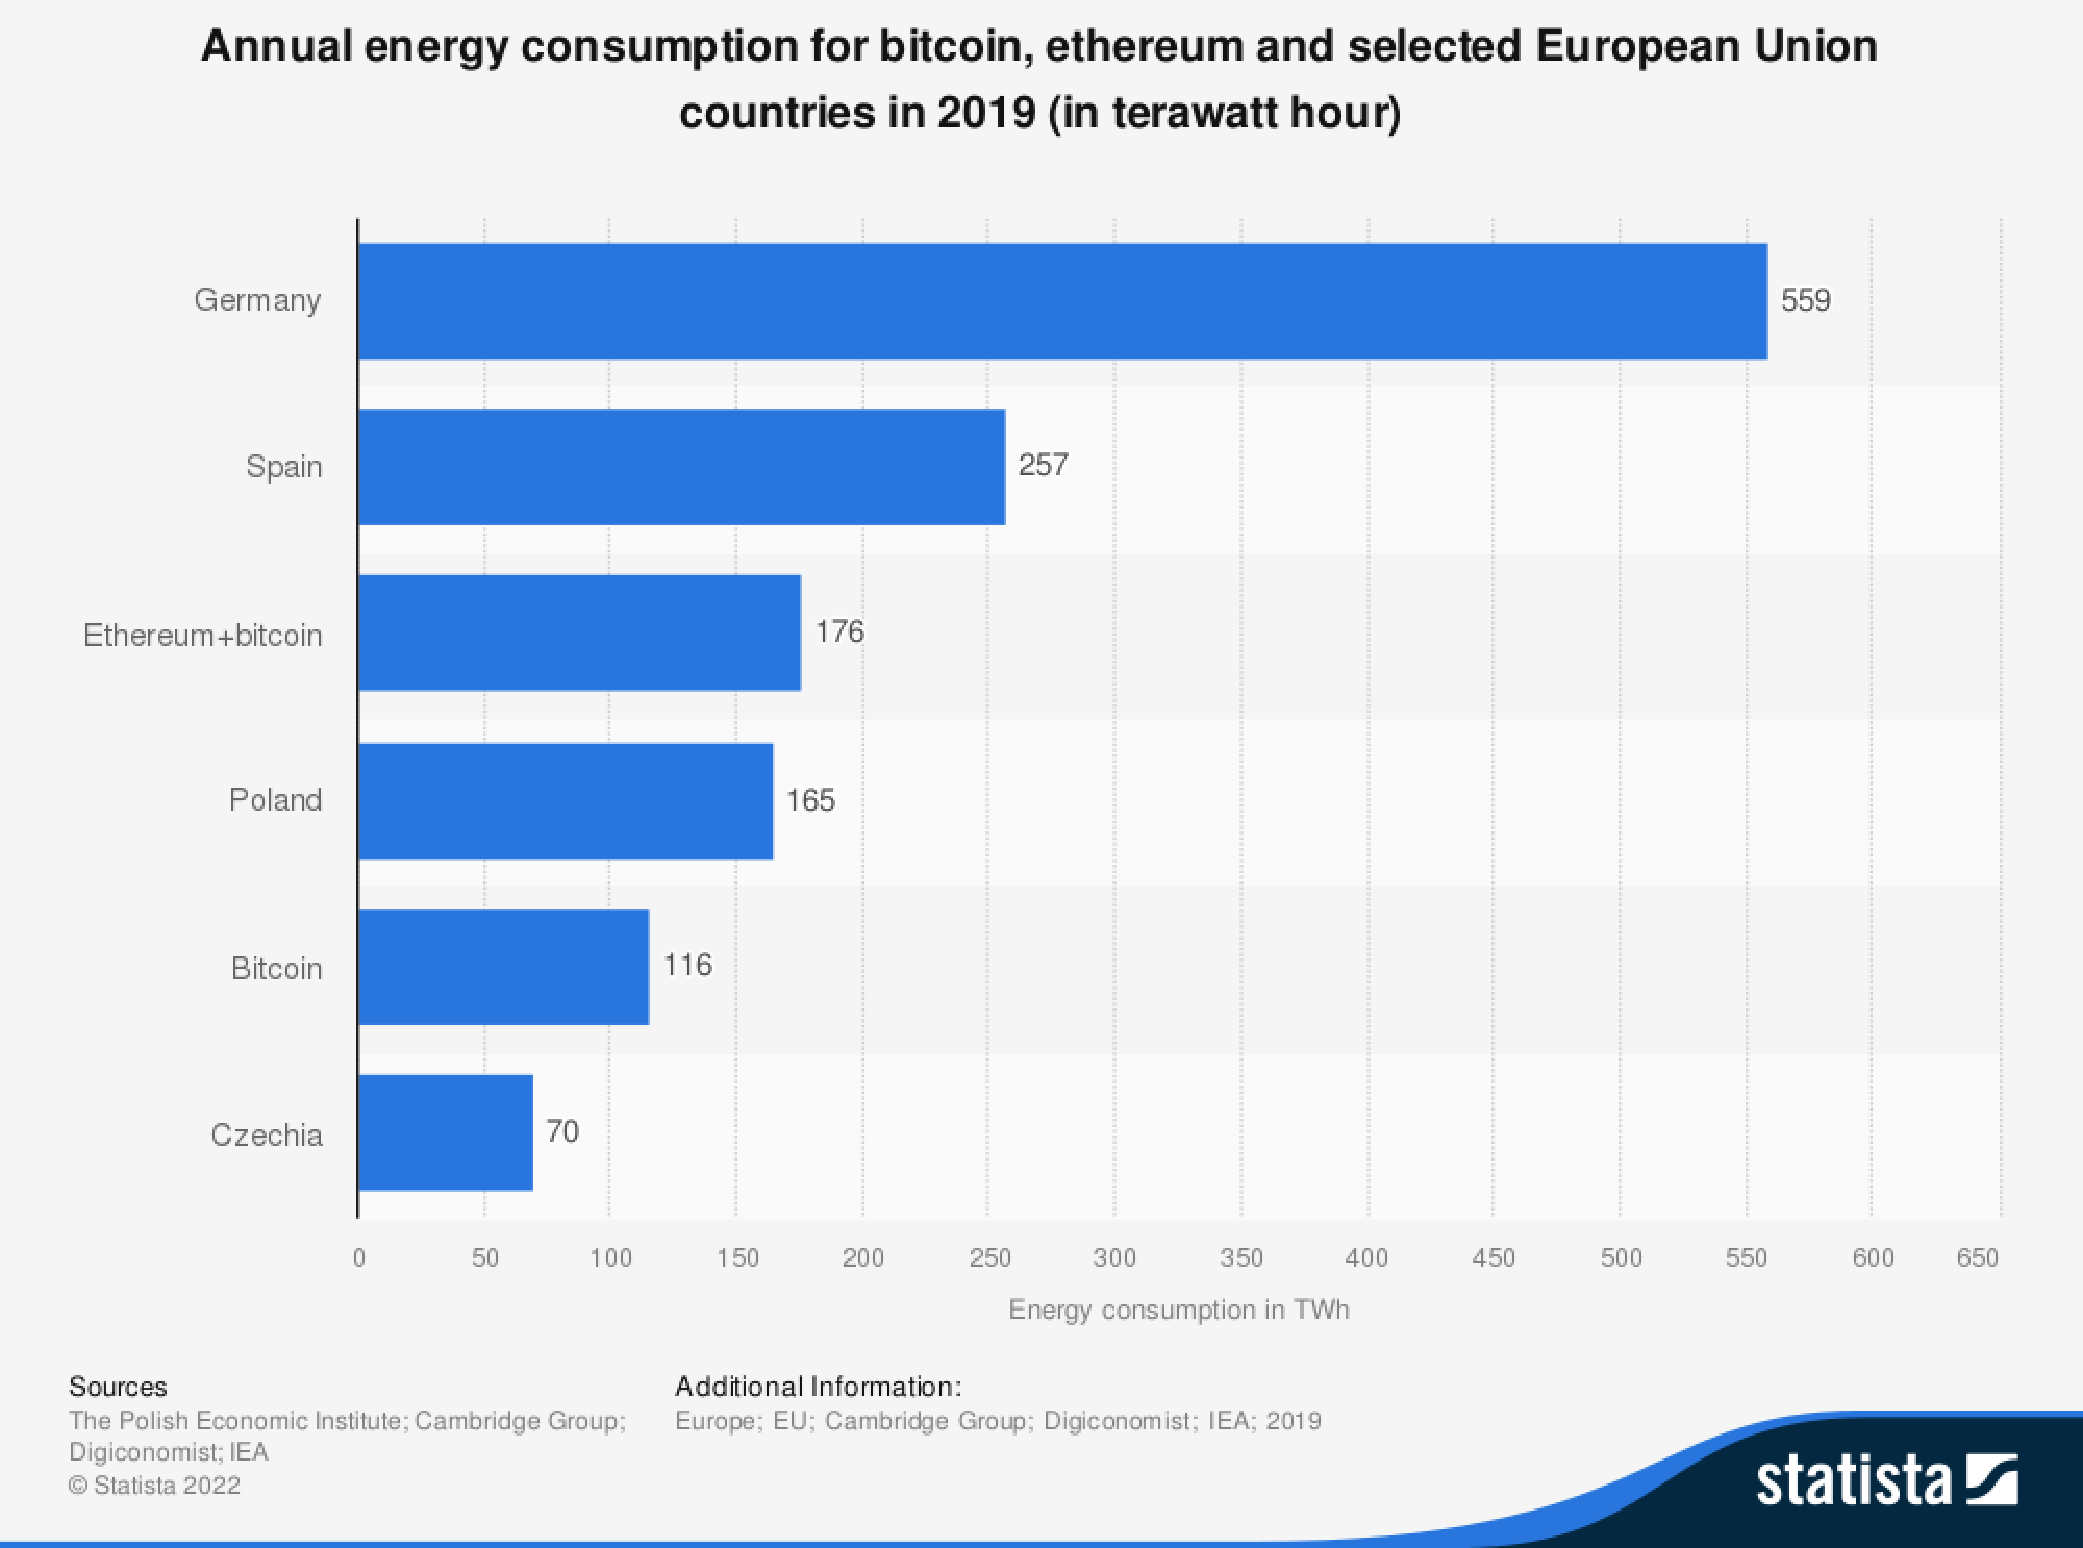
\includegraphics[scale=0.33]{Images/countries_BTC_ETH_energy.pdf}
        \caption{Annual energy consumption for bitcoin, ethereum and selected European Union countries in 2019 in terawatt hour \cite{PEI2021}}
        \label{F_countries_btc_energy}
        \end{figure*}

\section{Storage}

The Bitcoin blockchain has grown significantly since its inception to 475 GB as of June 8, 2023, and it continues to grow as new transactions are added to the network. Figure \ref{F_storage_btc} shows the evolution of Bitcoin's ledger size from 2009 to June, 2023. This continuous growth poses challenges for storage and synchronization for network participants. Running a full node, which stores a complete copy of the Bitcoin blockchain, requires substantial storage space. In addition to the blockchain data itself, a full node also needs to store additional data, such as transaction indexes and the UTXO set. As of now, a full node typically requires several terabytes of storage space.

\textbf{Pruning}. Bitcoin introduced a feature called pruning to address the storage requirements of running a full node. Pruning allows nodes to discard older blockchain data while still maintaining the ability to verify new transactions. This reduces storage requirements for nodes that do not need to maintain a complete history of all transactions.


\begin{figure*}[ht]
    \centering
     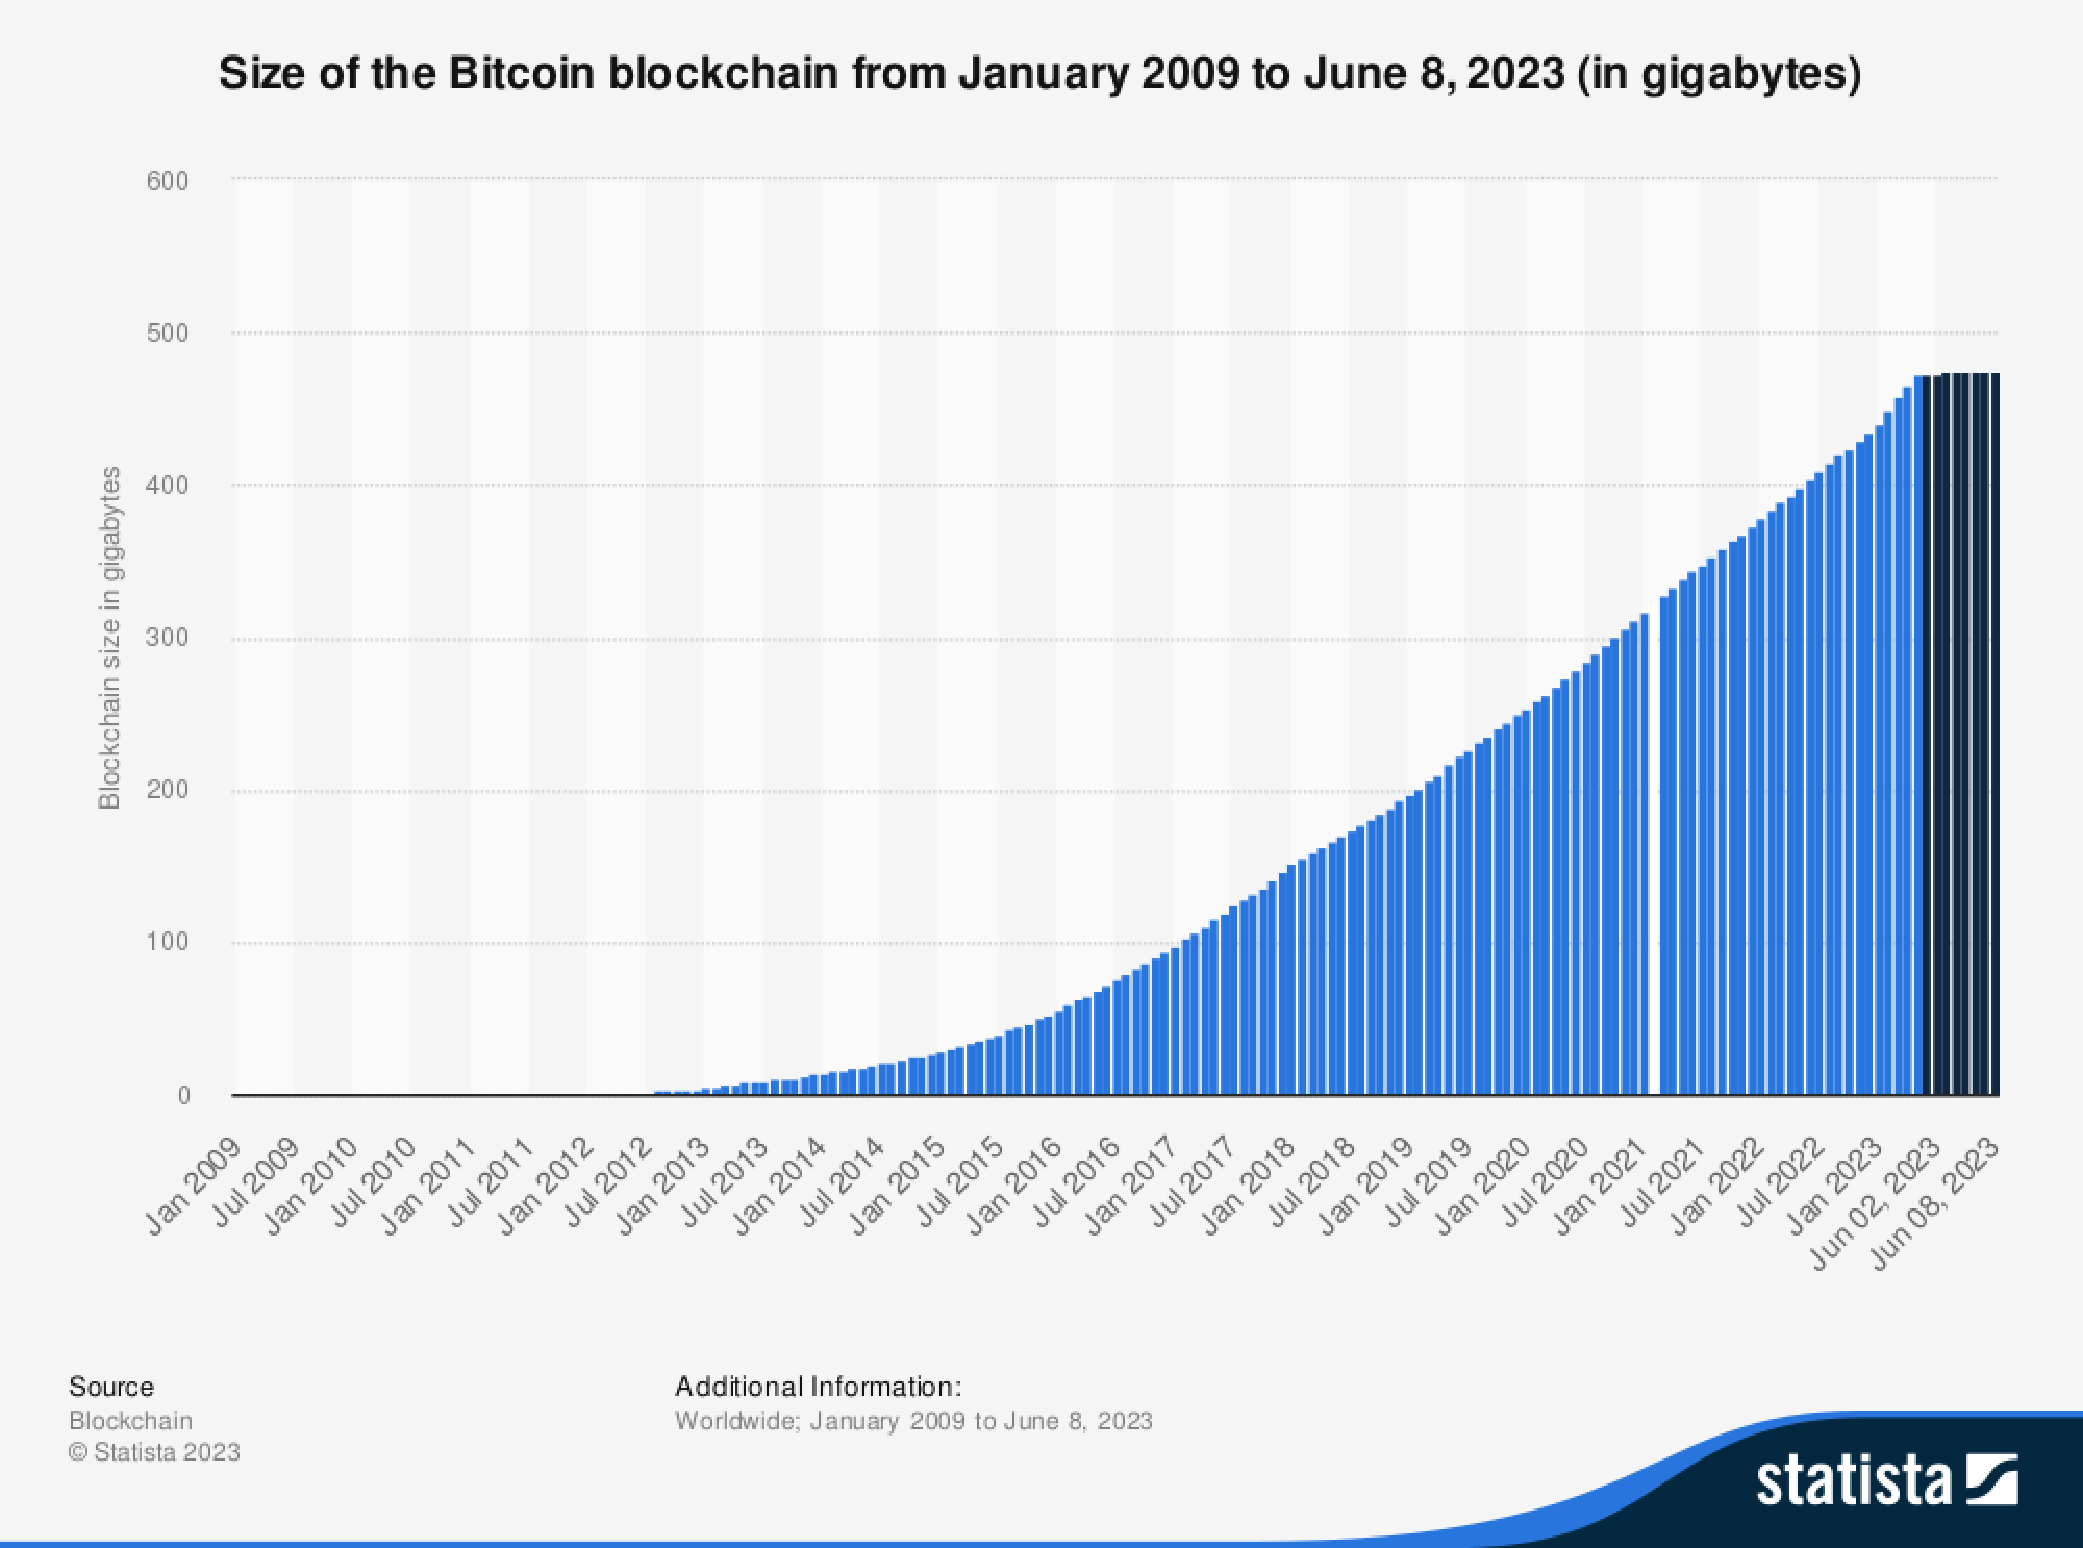
\includegraphics[scale=0.33]{Images/storage_btc.pdf}
    \caption{Size of the Bitcoin blockchain from January 2009 to June 8, 2023(in gigabytes) \cite{StatistaBTC2023}}
    \label{F_storage_btc}
    \end{figure*}